\chapter{Approach}

\section{System context}

The reimbursement-tool interacts with several user types as well as external software systems. In this section, these actors and software systems are introduced and resulting dependencies outlined.

\subsection{Actors}

The context diagram (see figure \ref{fig:context-diagram}) describes the relationships between the system and its users:
 \textit{Expense Creators}, in short creators, such as assistants, professors and the administrative employees can create expenses, view and print them. However, they are only allowed to modify their own expense while it is in the draft state i.e has not been submitted to the creator's manager yet.  \textit{Managers}, such as professors, the department manager and the head of IFI and the \textit{Finance administration} are able to \textit{reject expenses} and send them back to the \textit{Creator}. Besides rejecting expenses, they are also able to modify them. Moreover, \textit{Managers} have also to provide for each expense a project describtion. \textit{Guests} are allowed to view specific expenses and related expense-items too. However, they need the 32-character long internal expense \textit{Uid} to gain access to the expense's details. The \textit{Uid} is added on the printed expense document (see appendix \ref{sec:app-pdf}).

\subsection{Services}
The following sub chapters explain what interfaces to external service providers exist.

\subsubsection{IFI LDAP Server}
The reimbursement-tool fetches user-data from the IFI LDAP server (see figure \ref{fig:context-diagram}) and stores it in the reimbursement-database. By being able to reuse their existing LDAP credentials, users get a comfortable way to login to the system and ensures at the same time that only authenticated users gain access to the system. Furthermore, the user's current roles and the user's manager are assigned automatically. If there is no manager specified in the LDAP, a warning is shown to the user. For details about how to adjust the LDAP settings please refer to appendix \ref{subsubsec:ldap}.

\begin{figure}[H]
    \centering
    \fbox{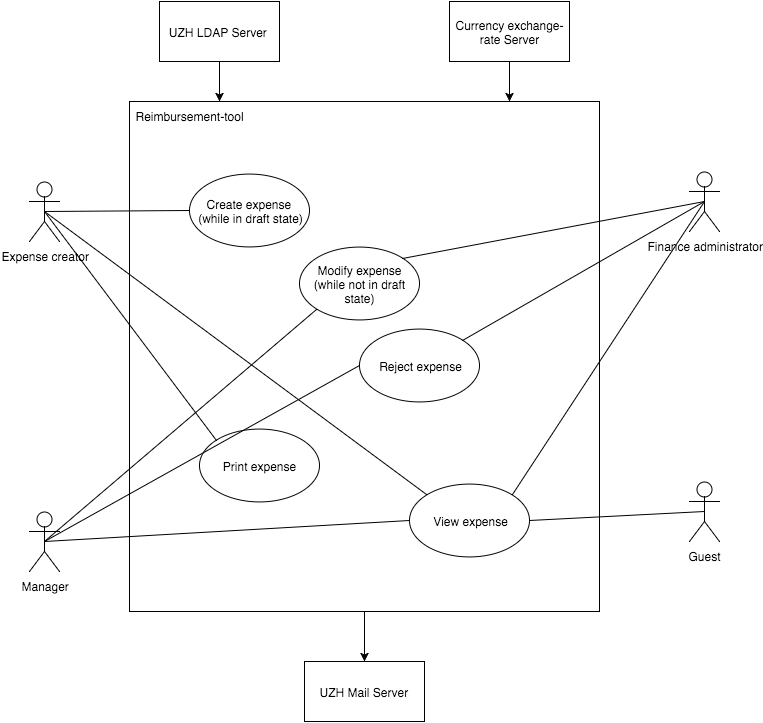
\includegraphics[width=0.80\textwidth]{context-diagram}}
    \caption{System context: Context diagram}
    \label{fig:context-diagram}
\end{figure}

\subsubsection{Currency exchange-rate Server}
Often expenses accrue in foreign currencies but are paid back in CHF. To provide the user with a handy but still accurate way to calculate the historically accurate amount that has to be charged back, the reimbursement tool integrates a currency-exchange-rate-service. We decided to use \textit{fixer.io} \cite{fixer} because it is free, updated daily, provides low response times and a high availability. While the \textit{European Central Bank(ECB)}\cite{ecb} is used as data source, \textit{fixer.io} provides a queryable webservice for it. Currently, the reimbursement-tool calls the API every time an exchange-rate is needed. For example if the user specifies the amount of a receipt in a foreign currency. Since the API is called by our reimbursement-server, any cheating regarding exchange rates is prevented.

\subsubsection{UZH Mail Server}
To notify users about actions that need their attention, the reimbursement-tool implements a notification algorithm. As soon as a new action has to be taken, the notification service adds the user's email address to the emailing list. Emails are sent out only three times a day (8am, 12pm and 5pm). At this points in time, the emailing list is processed by checking if there are still actions that need the user's attention. If that is the case, an email is sent out. If in the meantime the user took the required action, no email is sent out. If after an email sending no new action occurs that requires the user's attention, no reminder-email will be sent although there are remaining actions. For the actual email sending, the reimbursement-tool integrates the IFI Email Server. For more information about adjusting the e-mail settings please refer to appendix \ref{subsubsec:email}.

\newpage


\section{Architecture}

The back-end is considered as the software and database running on a Tomcat \cite{tomcat} server and uses PostgreSQL \cite{postgresql} to run the database on. The system is hosted by the IFI. The front-end/client communicates with the back-end using a RESTful service interface described in section \ref{sec:restfulapi}.

\subsection{Back-end}
The back-end is developed in Java. It is structured according to the rules of a multilayered software architecture. We use the domain driven design \cite{ddd} to apply commen patterns for the layers in the backend. The domain model, that consists of the concepts, is connected to the database. Changes on the model will be automatically synchronized with the database. The service package lists all methods that are used on a domain model.\newline
DTOs (Data Transfer Object) are used to transfers data from back-end to front-end and vice verse. \newline The implemented model- and service-classes are visualized in appendix \ref{sec:app-models} and \ref{sec:app-service}. \par

\subsection{Front-end}
The front-end is developed in JavaScript using the AngularJS \cite{angular} framework. AngularJS is based on an MVC (Model View Controller) pattern. It basically consists of controllers, templates used for the view, as well as models representing the data that is shown to the user using the templates. However, AngularJS \cite{angular} extends the basic MVC concept with useful enhancements like directives, filters, injectors etc. A complete list of the available concepts in AngularJS and small examples can be found at the AgngularJS: Developer Guide \cite{angular-devguide}.

\subsection{Multilayer architecture}
We use a common \textit{Multilayer architecture} (see figure \ref{fig:architecture-layer}) in the back-end to provide a good overview and maintenance of the entire software-code. The following four layers are used:
\begin{itemize}
    \item \textbf{Presentation Layer} provides the front-end code. It uses AngularJS for the GUI creation. The \textit{Presentation Layer} interacts with the \textit{Application Layer} using RESTful services.
    \item \textbf{Application Layer} provides the available services that interact with the \textit{Business Layer}. It hosts the Security, RESTful services and the Global Exceptions.
    \item \textbf{Business Layer} provides the available services that interact with the \textit{Data Access Layer}. It provides the relevant services and models based on the \textit{Data Access Layer}.
    \item \textbf{Data Access Layer} consists of repositories and the \textit{Hybernate} database.
\end{itemize}

\begin{figure}[H]
    \centering
    \fbox{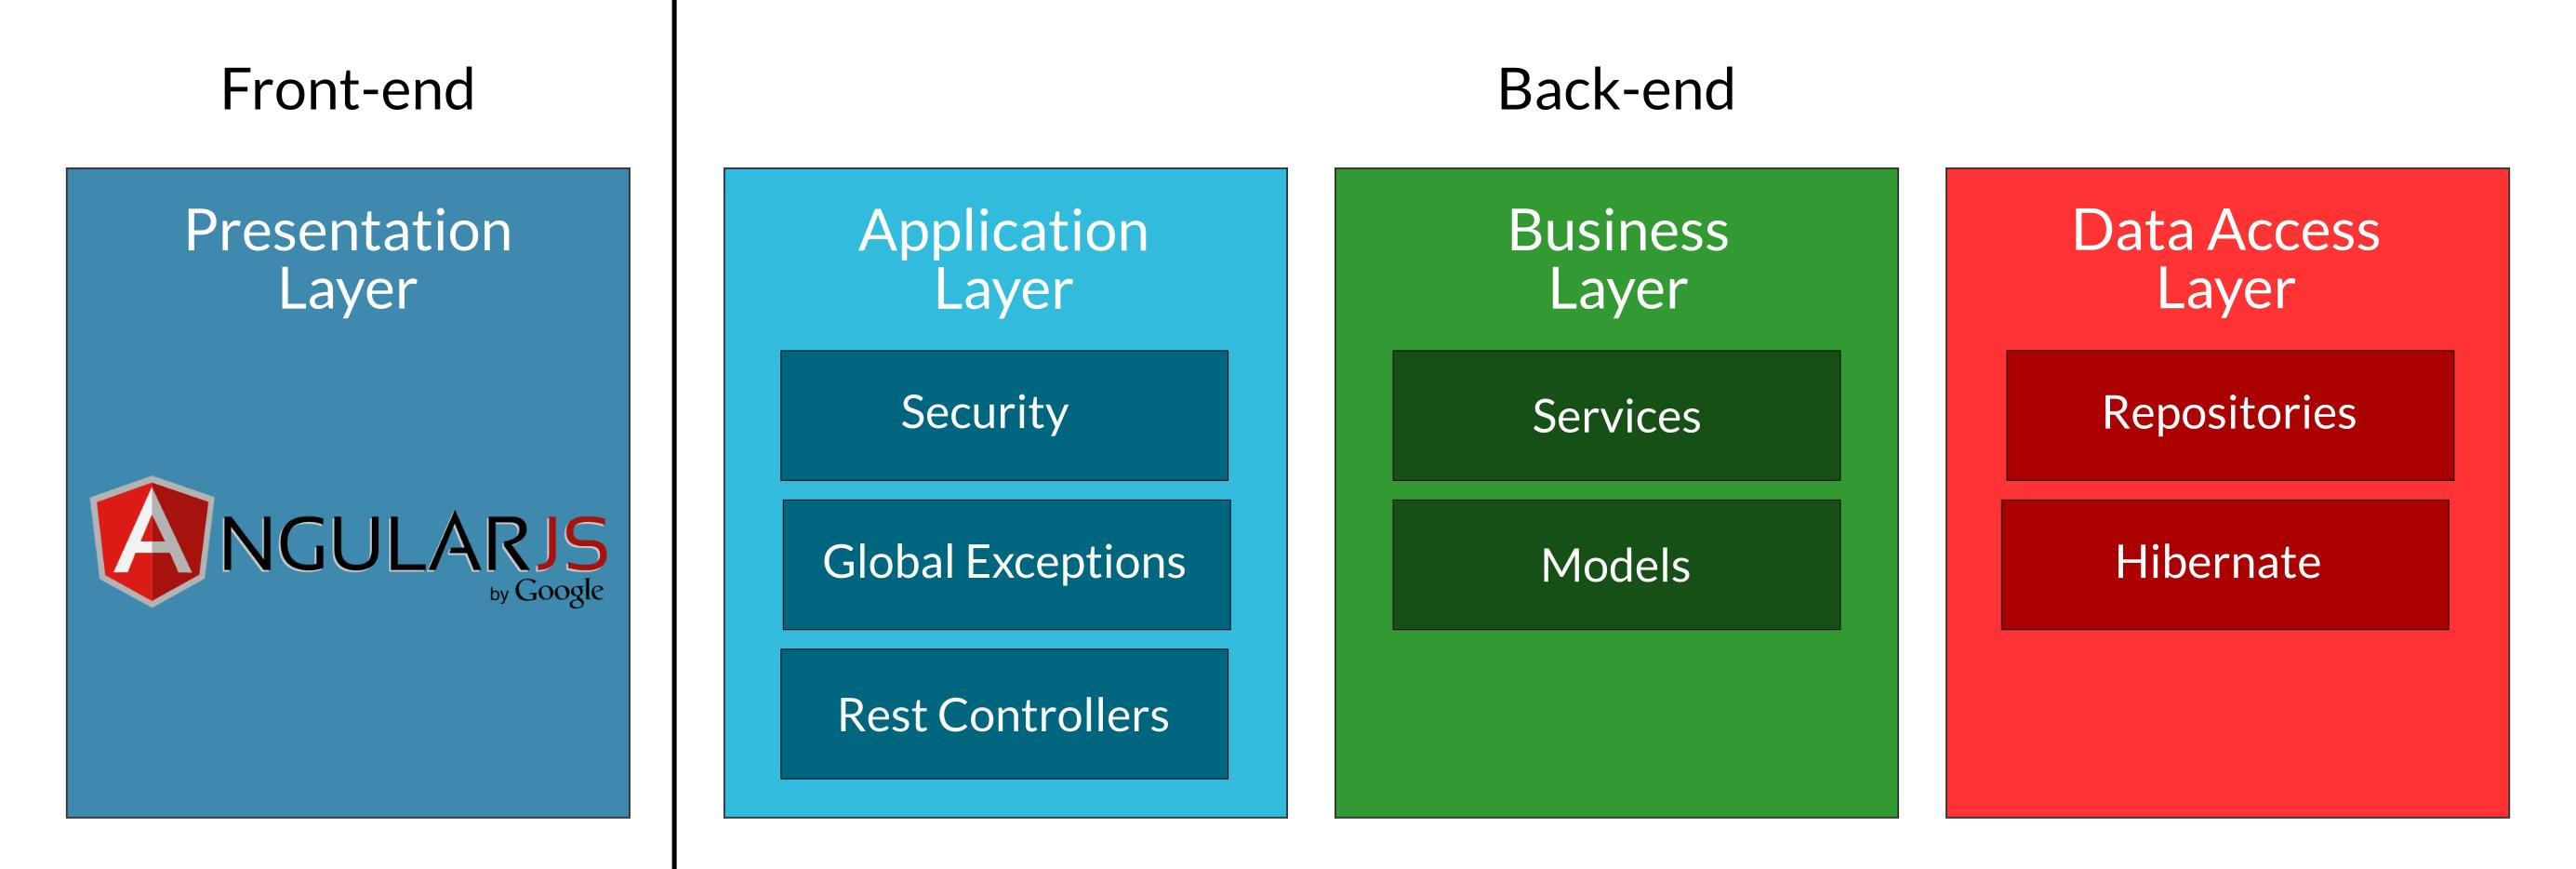
\includegraphics[width=0.80\textwidth]{architecture-layer}}
    \caption{Architecture: Multilayer architecture}
    \label{fig:architecture-layer}
\end{figure}

Our layers depend on each other while every layer communicates only with either the upper or the lower layer. This ensures a good maintainability and loose coupling of the single layers.\newline
For example: If the presentation layer needs to display an expense, the application layer will handle this request by first checking the relevant security parameter of the request followed by calling the business layer. The service will handle and aggregate the desired information fetched from the relevant models. In our case to display an expense, the service will retrieve all expense-items and expense-item-attachments.


\section{Processflow}
\label{sec:processflow}
As stated in section \ref{sec:states} an expense always has to be in one specific state. The entire process implemented in the system is documented in \ref{sec:process-diagram-rotated}.\newline
The process starts in the lane \textit{Employee}; an expense is created, receipts are added and it is forwarded to the next higher instance for verification. After the verifications by the \textit{Manager} or \textit{Department manager} and \textit{Finance administration} are successful, the signing-process will start. During the signing-process, all three entities; \textit{Employee}, \textit{Manager} and the \textit{Finance administration} need to sign the document. If all of them have signed the document correctly, the \textit{Creator} - the \textit{Employee} - can print the expense and hand it over physically to the \textit{Finance administration}. Currently this process step is not integrated in best practice. Because all of the expense receipts will be printed and after verification of the \textit{Finance administration UZH} it they will be digitalized again. This media disruption is also described in \ref{sec:future-work}.\par
However, corner-cases for example if a \textit{Manager} will act as a \textit{Creator} the expense will only be submitted to the \textit{Finance administration} for approval. However, during the signing-process the \textit{Manager} deputy has to sign as higher authority.

\subsection{States}
\label{sec:states}
During the process an expense passes through various states. An expense is always in one of the states defined followed. The State-diagram in \ref{sec:state-diagram} describes the expense transformation in viewpoint of states. Users have different roles and therefore have different authorizations to modify the state of an expense.

\begin{itemize}
    \item \textbf{DRAFT} state occurs if the expense is created and yet has not been assigned to a \textit{Manager}.

    \item \textbf{TO\_BE\_ASSIGNED} state occurs if the expense is submitted, but has not been assigned to a specific manager or the \textit{Finance administration} user. If the expense has been assigned, the expense will either have the state \newline \textbf{ASSIGNED\_TO\_MANAGER} or \newline \textbf{ASSIGNED\_TO\_FINANCE\_ADMIN}.

    \item \textbf{ASSIGNED\_TO\_MANAGER} state occurs if the expense is assigned to a specific \textit{Manager}.

    \item \textbf{ASSIGNED\_TO\_FINANCE\_ADMIN} state occurs if the expense is assigned to a specific \textit{Finance admin}.

    \item \textbf{REJECTED} state occurs if the created expense is not accepted by the \textit{Manager}, \textit{Department manager} or the \textit{Finance administration}. In \textbf{REJECTED} state the expense will be reassigned to the user who created it.

    \item \textbf{SIGNED} state occurs if the expense has been signed by all participants; \textit{Creator}, \textit{Manager} or \textit{Department manager} and \textit{Finance administration}. There exist sub states that occur if the expense is in the process of being signed:
        \begin{itemize}
            \item \textbf{TO\_BE\_SIGNED\_BY\_USER} occurs if the expense needs to be signed by the \textit{Creator}.
            \item \textbf{TO\_BE\_SIGNED\_BY\_MANAGER} occurs if the expense needs to be \newline signed by the \textit{Manager}.
            \item \textbf{TO\_BE\_SIGNED\_BY\_FINANCE\_ADMIN} occurs if the expense \newline needs to be signed by an user with role \textit{Finance administration}.
        \end{itemize}

    \item \textbf{PRINTED} state occurs if the expense and all its receipts are successfully converted into a digital document.

    \item \textbf{ARCHIVED} state occurs if the expense has been printed.
\end{itemize}

The names of the various states are coupled with the user roles. For example \textbf{ASSIGNED\_TO\_FINANCE\_ADMIN} implies that the expense is assigned to all users with roles \textit{Finance administration}.

\subsection{E-mail notification}
To inform the users of the reimbursement-tool about expense state changes, e-mail notifications have been implemented to notify affected users immediately. E-mail notifications are executed at the following actions:
\begin{itemize}
    \item An expense that has been created by a user and is assigned to a \textit{Manager}, will send an e-mail to the respective \textit{Manager}.
    \item An expense that has been approved by the \textit{Manager} and enters the state \newline \textbf{TO\_BE\_ASSIGNED}, will send an e-mail to all available users with role \textit{Finance administration}.
    \item An expense that needs to go through the signing process, will send an e-mail to notify every user who needs to sign the document.
    \item If an expense is rejected by a \textit{Manager} or the \textit{Finance administration} the \textit{Creator} of the expense will receive an e-mail notification.
\end{itemize}

E-mail notifications will be stored in a queue for each user and mailed to them three times a day in bulk mode. So we guarantee, that a user will not get spammed and the notifications messages are consolidated.

Besides state changes, e-mails will also be sent to an administrator if a general run-time exception occurs. To ensure the administrator of the reimbursement-tool is up-to date about major incidents.


\section{User roles}
\label{user-roles}

The system maps the users available in the IFI LDAP server. So every user that exists in the LDAP is capable to login to the system. He can use the same user name and password that he uses for the other University of Zurich services for login. \par

The reimbursement-tool provides different user roles. Also the roles on the reimbursement-tool are mapped with the LDAP user roles of the University of Zurich. So a user who is defined as professor for a specific group on the LDAP will be the manager for all users of this group. The reimbursement-tool provides the roles with the following authorizations to alter expenses:

\begin{itemize}
    \item \textbf{Unregistered user} are users, who are authorized to login the reimbursement-tool but have not yet completed the registration process. They have only access to the public REST services (see \ref{sec:rest-services}).
    \item \textbf{Registered user / User} passed the registration process. He can access the reimbursement-tool and create and manage his created expenses. He has one of the following roles:

    \begin{itemize}
        \item \textbf{Creator} is authorized to create and edit expenses as long as they are in DRAFT state.

        \item \textbf{Manager / Professor} are authorized to reject, accept and edit expenses as long as it is assigned to him.

        \item \textbf{Department manager} has the same authorizations as the \textit{Manager}. If a \textit{Manager} is outreach, his assignments will be forwarded to the respective \textit{Department manager}.

        \item \textbf{Finance administration} is authorized to reject, accept and edit expenses once they have been accepted by a \textit{Manager} or \textit{Department manager}. Furthermore they can manage the available cost categories and search for expenses.

        \item \textbf{Head of institute} has the same authorizations as the \textit{Manager}. In contrast to the \textbf{Department manager} there exists only one user that can be \textit{Head of institute}. The \textit{Head of institute} will have to approve the expense if, for any reason the \textit{Department manager} is not available.
    \end{itemize}
\end{itemize}


\section{Technologies}

In the following section the technologies used are being described and explained why they had been chosen.

\subsection{Back-end}

\subsubsection{Java}
The reimbursement-tool uses Java SE 7 for the back-end programming language. Java is an industry wide standard, has detailed documentation and there is sufficient knowledge at the IFI department to guarantee an adequate support and further development of the software.

\subsubsection{Hibernate}
\textit{Hibernate} abstracts the data layer. So that SQL-queries have to be written in rare cases only, which increases the code-clarity and decreases the code-complexity. All data operation are handled implicitly by defined Java data classes.\newline
H2 database is a temporary database for storing data in a database environment. It offers a simple interface and can be used for development, given that only one development database server is available. \cite{hibernate}

\subsubsection{Java Spring Framework}
We decided to use the \textit{Spring Framework} because it's well documented, widely used and easy to integrate in an existing Java project. Therefore we use various components of the Java Spring Framework \cite{spring}:
\begin{itemize}
    \item Spring Security for the login- and user-management as well as role based access-management for the RESTful resources.
    \item Spring Web MVC framework used to define RESTful interface within a few lines of code.
    \item Spring ORM used for the XML mapping within the process of Pdf-generation.
    \item Spring data is used to provide a simpler method to use data access technologies. It uses the DAO (Data Access Object) \cite{dao} to access data in a standard database like SQL.
\end{itemize}

\subsubsection{Maven}
The tool uses Apache Maven \cite{maven} for the build process and dependency management. We decided to use it, because it is widely used and is easy to maintain with a single \textit{pom.xml} file.

\subsubsection{Apache FOP}
The generated Pdf by the reimbursement-tool needs to be identical to the existing MS-Office Excel-Pdf file provided by the Finance Administration of the University of Zurich. The generated Pdf structure is added in \ref{sec:app-pdf}.\newline
The Pdf gets generated using an individual created XSLT template and a XML document generated out of a Java Object. Combining these two files generates an \textit{.fo} document, which will be used by Apache FOP \cite{apache-fop} to generate the Pdf.\par
We decided for Apache FOP because it is based on widely used standards like XML and XSL so that ongoing maintenance can be achieved easily and without specific knowledge required.

\subsubsection{Digital signature}
The ability to sign the printed Pdf document is crucial so that authenticity is provided. Especially if the Pdf document will be used as evidence by the Finance Administration of the University of Zurich. The system provides two types of signatures \cite{arx-signature}:
\begin{itemize}
    \item A \textbf{Digital signature} ensure the authenticity of the signer. Any changes made to the document after it has been signed will invalidate the signature. To use it the user has to provide his private key to successfully sign the document.
    \item \textbf{Electronic signature} does not ensure the authenticity of the signer. Anyone can theoretically make changes on the document after it has been signed without the signature become invalid. The handwritten signature captured during the registration will be stamped on the Pdf document.
\end{itemize}\par

The implementation of the digital signature is done using a third party library pdfsign.js \cite{pdfsign} that allows us to do the pdf signing in the browser and not on the server. Due to the requirement, that the private key cannot be uploaded or processed by the server, the signing needs to be done on the client using the web browser.\par

All involved participants need to sign the document; \textit{Creator}, \textit{Manager} and the \textit{Finance administration} to proof their acceptance of the expense and the captured receipts. \par

\subsection{Interface}

\subsubsection{RESTful API}
\label{sec:restfulapi}
The tool uses a RESTful API that provides services to access the back-end resources. It is implemented using the Spring MVC. /newline
The available methods provided by the backend are listed in \ref{sec:rest-services}. There exist private and public services. Private services can only be access by a \textbf{Registered user / User} (private services are marked with the term PRIVATE).

\subsubsection{Swagger UI}
The Swagger UI visualizes all methods provided by the RESTful interface using a simple GUI. Furthermore developers can interact directly with the Swagger UI to test the \texttt{HTTP} methods. Figure \ref{fig:swagger01} shows a screen-shot of our Swagger UI. It visualizes all the available methods for the \texttt{public} resource as well as the mandatory and optional parameters for \texttt{HTTP} calls. This was important for the process of development. \cite{swagger} \par
We decided on Swagger UI, because a simple and easy to understand overview, as well as a simple integration into the software source-code. Further testing the back-end functionality was very simple using Swagger UI.

\begin{figure}[H]
    \centering
    \fbox{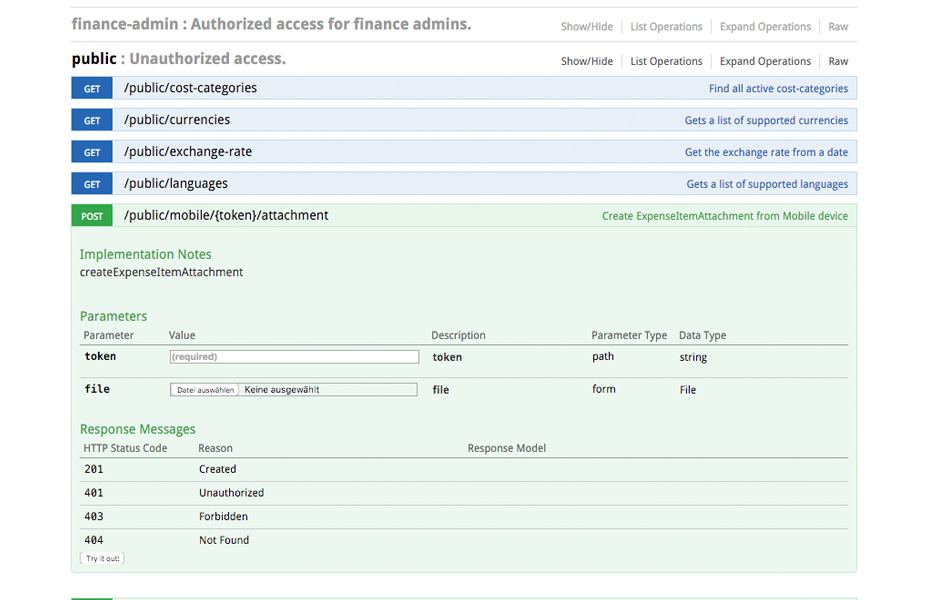
\includegraphics[width=0.80\textwidth]{swagger01}}
    \caption{Swagger: Reimbursement GUI}
    \label{fig:swagger01}
\end{figure}

\subsection{Front-end}

\subsubsection{AngularJS}
The tool uses the AngularJS framework. Its data bindings and dependency injections reduces the amount of code need to be written. Further it uses HTML templates and an sophisticated routing concept to deliver interactive GUIs. AngularJS is based on an MVC approach and is easy to integrate with REST services.\cite{angular}\par
We used AngularJS because of its broad community and the fact that it's supported by Google makes it future-proof.

\subsubsection{Bootstrap}
Bootstrap is a framework that consists of HTML, CSS and JavaScript elements. It can be used to create appealing responsive websites. Further it's CSS elements are supported by most of the desktop and mobile web-browsers available. The tool uses Bootstrap v. 3.3.5. \cite{bootstrap}\par
We use Bootstrap to speed-up the GUI development process. Using the elements it provides makes it easy to setup a responsive website within minutes. Further it provides a lot of fancy HTML/CSS elements like \textit{accordions}, \textit{modals}, etc.

\subsubsection{Bower}
The tool uses Bower for the client-side package management. Bower is a package manager for JavaScript web applications like AngularJS. It keeps track of the used assets, frameworks, libraries, etc. \cite{bower} \par
We used Bower because of its widely used, has a sound documentation and is easy to work with.

\subsubsection{Grunt}
Grunt is a JavaScript task runner. We use it for our client-side build. Its plugin directory supports a lot of modules to optimize the development work flow. Code-uglifying, concating, sass-compiling, file operations, auto prefixing etc. \cite{grunt} \par
We used Grunt because its widely used and there exists sound know how about its usage in our team.
